\documentclass[10pt]{article}

\usepackage{fullpage}
\usepackage{amsmath}
\usepackage{amsthm}
\usepackage{url}
\usepackage{relsize}
\usepackage{xspace}
\usepackage{subfigure}
\usepackage{graphicx,color}
\usepackage{amssymb}
\usepackage[margin=0.82in]{geometry}

\def\TODO#1{\noindent\textbf{[TODO: #1}]}

\begin{document}
\title{Predicting the Stock Market with Newspaper Articles\\ (6.867 Final Project)}
%\subtitle{6.867 Final Project}
\author{Chris Johnson \and Fredrik Kjolstad}
\date{December 10, 2012}
\maketitle

\begin{abstract}

\end{abstract}

\section{Introduction}

\section{Feature Selection}

Our data set consists of 36,466 Wall Street Journal (WSJ) articles over 359 days, and 251 days of closing price information of the Dow Jones Industrial Average (DJI) for the year 2007. The stock market is closed on weekends and holidays, which is why there are fewer days of stock data than newspaper articles. There are two days for which we have stock data but no newspaper articles (December 18th and 27th), but this appears to be an omission in the provided data set. We consider only days for which we have both WSJ and DJI data. 

We have approximately 101 articles per day on average. A histogram of articles per day appears in Figure~\ref{articlehist}. The distribution appears to be bimodal, with numbers of articles around either 125 or 15 per day. Since some days have fewer articles, which may decrease their effectiveness for classification. 

\TODO{Maybe we want to scale counts per day, but for NB this doesn't matter. Maybe some of the dimensionality reduction techniques are returning which days have more articles!}

\begin{figure}
\centering
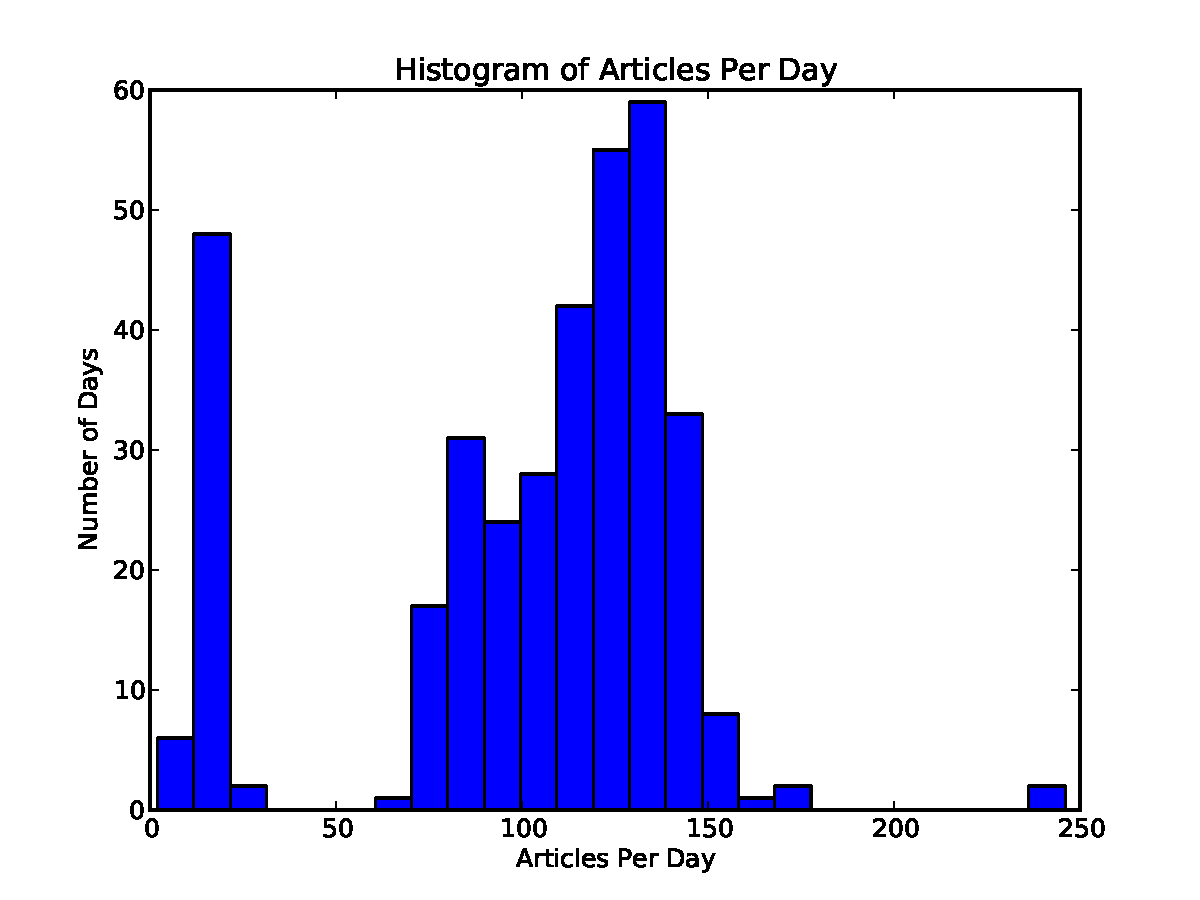
\includegraphics[scale=0.3]{text/articleshist.pdf}
\caption{Histogram of Articles Per Day}

\label{articlehist}
\end{figure}

Our data set consists of over 24 million words, with an average of 667 words per article. A histogram of article lengths appears in Figure~\ref{wordshist}. Most articles tend to be less than 2000 words, but there appears to be a long tail consisting of a few very long articles. For the most part it appears that article lengths are similar apart from a few outliers.


\begin{figure}
\centering
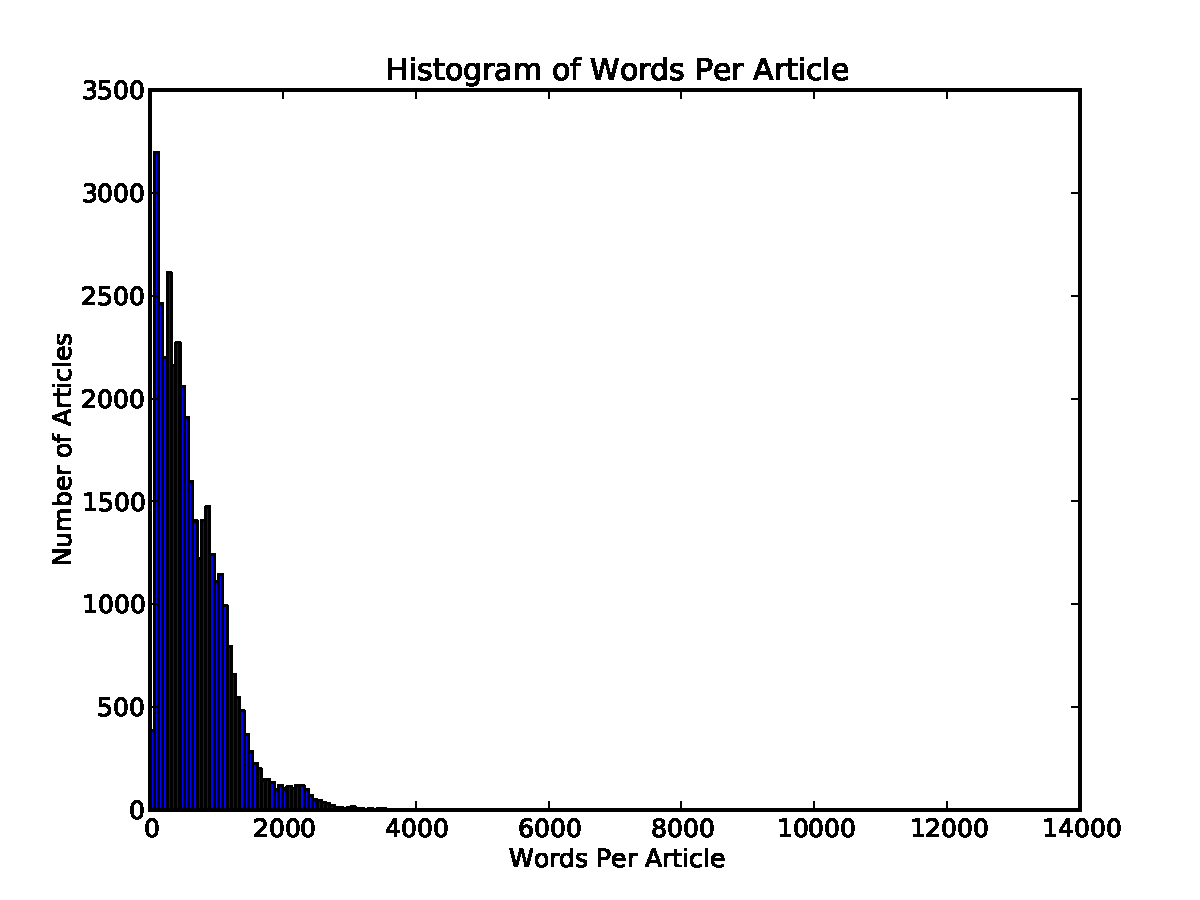
\includegraphics[scale=0.3]{text/wordshist.pdf}
\caption{Histogram of Words Per Article}
\label{wordshist}
\end{figure}

The data set contains 150,875 unique words. Each data point we use for training and validation therefore consists of a class label (+1 if the market went up that day, -1 if it went down) and a feature vector computed using frequencies of these unique words.

Due to the difficulty of computation on the number of unique words that we have, we filter the words in several ways to reduce the noise of the data set. First, we strip all non-alphabetic characters from all words and filter out any words less than length 2. We then filter out any words that did not appear more than some cutoff, $m$, throughout the year. We assume that these words are either misspellings or words which would not generally be useful in predicting stock performance due to their infrequency. Filtering with $m = 10$ results in 44,218 unique words and was found to be a good balance between information and computational tractability.
Finally, we filtered out any of the 100 most commonly used English words~\footnote{http://en.wikipedia.org/wiki/Most\_common\_words\_in\_English}, since we
assume that words such as ``and'' and ``I'' do not provide very much information.

We use several feature extraction techniques to construct the data matrix $F$. Each row of $F$ is the feature for a corresponding day, and each column of $F$
contains the values for one feature across all days. The column-vector $Y$ contains the output values (+1 or -1). 

The rest of this section describes several feature extraction techniques we used and the representation of the feature matrix $F$.  These features are compared using several machine learning algorithms presented in Section~\ref{sec:techniques}.

We will introduce the following terminology to describe the feature matrix and its elements:

\begin{itemize}


\item $F_{d,i}$ is the ith element of the feature vector for day $d$.

%\item $W$ is a vector with a count for each word over the entire year. Thus, $W_i$ is the number of times word $i$ appeared in the year.  

\item $A$ is a vector of word counts for a single article. Thus, $A_i$ is the number of times word $i$ appeared in article $A$.

\item $D$ is a vector of days, each element of which is a set of articles. $A \in D_k$ if and only if article $A$ was published on day $k$.


\end{itemize}

\subsection{Bag of Words and Phrases}

The simplest feature vector is simply a ``bag of words'' for each day~\cite{featurehash}, which consists of frequency counts of all words in articles published on that day. Elements of the feature vector take the form: $$\displaystyle F_{d,i} = \sum_{A \in D_d}{A_i}$$ These feature vectors are extremely sparse, since most articles do not use tens of thousands of unique words (we represent our data set as a sparse matrix
in MATLAB to reduce memory consumption to reasonable levels).

An obvious weakness of this technique is that it takes words out of context. Phrases such as ``stocks went up'' simply increase the counts of the three words independently. We augmented this technique by creating ``bags of phrases'' as well. In addition to counts of words, we keep counts of two and three word phrases
as well. We turn phrases into single words of the form ``word1-word2'' and ``word1-word2-word3'' with the restrictions that word1 and word3 may not be common words and the first or last words of a phrase may not be a single character. Common words beginning a 2 word phrase or ending a 3 word phrase are undesirable because we want to pick up on phrases where the subject is important. The middle word in the 3 word phrases may be common so we find phrases that combine two useful words such as, ``stocks are down.'' Filtering out phrases that appear less than $m = 10$ times in the year results in 194,679 unique phrases and words, so this technique can greatly increase the number of features.

Bags of words and bags of phrases form the basis of many of our other feature selection techniques, so we will call the feature matrix resulting from the use of either $B$. Since bags of phrases just increase the vocabulary size, it can be viewed as augmenting the article word lists $A$ with additional words. They bags of words or phrases may be used interchangeably, so we will refer to the resulting feature matrix for either as $B$ in the rest of this section; when we present results we will explicitly state if we build on bags of words or phrases as well as the filtering parameters used.

\subsection{Temporal Features}

Temporal shifting trades information about the current day for information about the previous (or next) day.

%To find a correlation from this would mean one of three things: that the market is influenced by the content of the WSJ on that day (perhaps investors read the paper in the morning and this influences how they trade throughout the day), that the content of the WSJ is influenced by the market on that day (impossible, because the newspaper is released before the market opens), or that some hidden ``state of the world'' influences both the newspaper and the market. 


\subsection{Topic Modeling}

 
\TODO{Read the paper that is cited and see if implementing hashing is good, seems our assumptions are different from theirs}

\TODO{Exhaustively discuss all feature selections here and cite sources}

\TODO{Read all sources and be familiar with them for interview!}
 

\section{Classifiers}
\label{sec:techniques}

In this section we describe and briefly evaluate the different classifiers we developed for this project.
For each classifiers we describe our implementation choices, what if any third-party libraries we used, and then we demonstrate its performance on our dataset.

Our classifiers can roughly be divided into four categories. The first are simple prediction rules. These are mostly included to demonstrate features of our data and to serve as baselines for the other classifiers. The next class include classifiers that do not have a probabilistic model. These include AdaBoost, Nearest Neighbor and SVM. The third class consist of classifiers based on probabilistic models. The only classifiers we implemented in this category is Naive Bayes. The fourth and final class of classifiers is sequential models and include M-order Markov Models and Hidden Markov Models.



\subsection{Prediction Rules}
\label{sec:prediction-rules}

In order to demonstrate properties of our data and to serve as baselines for more sophisticate classifiers we experimented with three simple prediction rules.

\begin{description}
\item[Majority] The first prediction rule is simply to count the number of positive and negative days in our training data set and 
\end{description}


\subsection{AdaBoost}
\label{sec:adaboost}

\subsection{Nearest Neighbor}
\label{sec:nearest-neighbor}

\subsection{SVM}
\label{sec:svm}

\subsection{Naive Bayes}
\label{sec:naive-bayes}

\subsection{Sequential Models}
\label{sec:sequential-models}

\subsubsection*{Markov Models}
\label{sec:}

\subsubsection*{Hidden Markov Models}
\label{sec:}

\section{Analysis}

\subsection{Temporal Shift}

The bag features $B$ associate each day's price direction in $Y$ with the same day's article counts, so we are using that feature matrix to find a correlation between the direction of the stock market and the contents of newspaper articles on day $d$ (perhaps investors read the paper in the morning and that influences their trades, or some hidden ``state of the market'' influences both). It is plausible, however, that the articles on day $d-1$ are correlated with the market direction on day $d$. It is also likely that the articles on day $d+1$ are correlated with the market direction on day $d$, since they may reflect on market performance for the previous day. This is an uninteresting predictor, but it will give us some indication of how well the techniques we apply make predictions based on data that has a clear reason for being correlated.

We introduce temporally shifted feature matrices to investigate these possibilities, defined by $F_{d,i} = B_{d-1,i}$ and $F_{d,i} = B_{d+1,i}$ That is, each count is replaced either by the previous day's count or the next day's count. The first and last days' counts will be 0 respectively, so this loses some information for one day each.

\begin{itemize}
\item The word ``ambitions'' is the best indicator of the Dow Jones gaining. If ``ambitions'' appeared in the WSJ there was a 64.26\% chance that the Dow Jones went up on that day.
\item The word ``tundra'' is the best indicator of the Dow Jones falling. If ``tundra'' appeared in the WSJ there was a 64.26\% chance that the Dow Jones fell on that day. This is because a series of articles in the WSJ where they talk about how Toyota is producing more cars outside the us and where they mention the Toyota Tundra. Another item is how Toyota is passing GM in sales (tundra is mentioned). A third item is about how Tundras had to be discounted (Toyota is on the Dow Jones).

\end{itemize}

\bibliographystyle{plain}
\bibliography{report.bib}

\end{document}
